\documentclass[11pt]{article}

\usepackage[a4paper, margin=0.9in]{geometry}
\usepackage{amsmath, amssymb}
\usepackage{graphicx}
\usepackage{booktabs}
\usepackage{array}
\usepackage{multirow}
\usepackage{enumitem}
\usepackage{xcolor}
\usepackage{caption}
\usepackage{subcaption}
\usepackage{float}
\usepackage{tikz}
\usetikzlibrary{positioning, arrows.meta, fit}
\usepackage[colorlinks=true, linkcolor=blue, citecolor=blue, urlcolor=blue]{hyperref}
\captionsetup{font=small, skip=4pt}
\setlength{\textfloatsep}{8pt}\setlength{\floatsep}{6pt}\setlength{\intextsep}{6pt}
\setlist{itemsep=1pt, topsep=2pt}

\newcommand{\todo}[1]{\textcolor{red}{\textbf{[TODO: #1]}}}

\title{\textbf{CS781 Capstone Final Report}\\[3pt]
\large Four From-Scratch Indian-Legal Language Models and Their Seven Task Descendants}
\author{Kartik Agrawal \\ Roll number 240526 \\ Codabench: \texttt{k\_240526}}
\date{9 November 2026}

\begin{document}
\maketitle

\begin{abstract}
We built a complete Indian-legal NLP pipeline under the CS781 capstone constraints: every model starts from a language model we pretrained ourselves (50--300M parameters, no pretrained weights), and all training ran on free Kaggle T4 GPUs. In Phase~1 we trained four architectures with one shared 32k byte-level BPE tokenizer: a 12-layer prefix language model, a 6+5-layer encoder--decoder, a 9-layer multi-scale retention model and a 16-layer ``Bi-Scale'' model with grouped-query attention and local/global layers. In Phases~2--7 we adapted these backbones to legal NER, rhetorical-role labelling, judgment prediction, statute identification, abstractive summarization and prior-case retrieval, comparing full and partial fine-tuning, LoRA, rsLoRA, LoRMA, BitFit, Houlsby and Pfeiffer adapters, prefix and prompt tuning, and knowledge distillation (KD) in at least six runs per phase. Our best Codabench scores are 0.835 BERTScore (Phase 1), 0.513 strict macro-F1 (NER), 0.494 macro-F1 (rhetorical roles), 0.622 (judgment prediction), 0.358 (statutes), 0.833 BERTScore (summarization) and 0.259 Micro-F1@7 (retrieval). Two findings recur across phases: the bidirectional prefix-LM was the most reliable backbone for representation tasks, and KD students kept most of their teacher's score with fewer layers; methods that freeze the encoder--decoder's encoder and train only a few parameters were consistently the weakest.
\end{abstract}

%=====================================================================
\section{Competition Result}
\label{sec:competition}
\textbf{Codabench username:} \texttt{k\_240526} \quad \textbf{Roll number:} 240526 \quad
\textbf{GitHub:} \url{https://github.com/Luciferk07/cs781-capstone}

\begin{table}[H]
\centering\small
\caption{Official leaderboard results (best submission per phase).}
\label{tab:leaderboard}
\resizebox{\linewidth}{!}{\begin{tabular}{llcccl}
\toprule
\textbf{Phase} & \textbf{Primary metric} & \textbf{Score} & \textbf{Rank / participants} & \textbf{Valid subs.} & \textbf{Best submission} \\
\midrule
1 Legal LM            & BERTScore F1        & 0.8347 & 39 / 142 & 7 & \texttt{submission-arch4} (Retention) \\
2 Legal NER           & strict macro-F1     & 0.5126 & 74 / 133 & 6 & \texttt{prefixlm\_lorma\_viterbi} \\
3 Rhetorical roles    & macro-F1            & 0.4941 & 68 / 132 & 6 & \texttt{r1\_lorma\_prefixlm} \\
4 Judgment prediction & macro-F1            & 0.6224 & 115 / 132 & 9 & \texttt{r6\_kd\_student} (Prefix-LM) \\
5 Statute identif.    & macro-F1            & 0.3582 & 88 / 133 & 8 & \texttt{r8\_full\_prefixlm} \\
6 Summarization       & BERTScore F1        & 0.8333 & 89 / 131 & 7 & \texttt{r2\_lora\_prefixlm} \\
7 Prior case retrieval& Micro-F1@7          & 0.2593 & 114 / 133 & 6 & \texttt{p1\_full} (Prefix-LM) \\
\bottomrule
\end{tabular}}
\end{table}
\noindent Total valid submissions: 49 (one further Phase-2 submission failed scoring). \qquad Scores and ranks recorded on 9 November 2026.

%=====================================================================
\section{Introduction and Problem Description}
\label{sec:intro}
Indian court judgments are long (a median of 3.7--5.8k tokens in Phases 6--7, with tails beyond 100k), formulaic in parts (headers, citations, statute references) and written in a register that general-purpose models handle poorly. The capstone asks whether a compact model trained only on the released legal corpus can support the whole range of legal NLP tasks. The task suite (Table~\ref{tab:tasks}) follows IL-TUR \cite{joshi2024ilTUR}.

\begin{table}[H]
\centering\small
\caption{Tasks and primary metrics.}
\label{tab:tasks}
\resizebox{\linewidth}{!}{\begin{tabular}{llll}
\toprule
\textbf{Phase} & \textbf{Input} & \textbf{Output} & \textbf{Metric} \\
\midrule
1 Pretraining & Acts, Supreme Court, High Court, Tribunal corpora; 512-word test prompts & 128-word continuation & BERTScore F1 \\
2 L-NER & judgment text (character offsets) & spans of 12 entity types & strict macro-F1 \\
3 Rhetorical roles & judgment as a sentence list (Corporate Law, IT) & one of 13 roles per sentence & macro-F1 \\
4 CJPE & full judgment & accepted / rejected (1/0) & macro-F1 \\
5 LSI & case facts & subset of 100 statute ids & macro-F1 \\
6 Summarization & judgment & abstractive summary & BERTScore F1 \\
7 PCR & query judgment + candidate pool & 7 ranked candidate ids & Micro-F1@7 \\
\bottomrule
\end{tabular}}
\end{table}

\paragraph{Constraints.} The Phase-1 model has 50--300M parameters and is trained from scratch; no pretrained language model, pretrained weights or external LLM API may be used; Phases 2--7 start from a Phase-1 checkpoint; each of Phases 2--7 needs at least six substantially different submissions; compute is free Kaggle/Colab GPUs (two T4s, 12-hour sessions).

\paragraph{Questions we investigated.} (i) Which of four architecturally different Phase-1 models transfers best, task by task? (ii) Under a fixed time budget, how do parameter-efficient methods compare with full and partial fine-tuning? (iii) How should long documents be cut to fit a 1{,}024-token context (head, tail, head+tail, multiple chunks)? (iv) How much do decoding choices matter: Viterbi decoding for NER, dev-tuned thresholds for CJPE and LSI? (v) How much does a KD student with fewer layers lose?

\paragraph{Scope.} We built the tokenizer, four Phase-1 models and seven task pipelines end to end. We did not attempt QLoRA, IA$^3$ or AdaLoRA, cross-encoder re-ranking for retrieval, ensembling, or reinforcement-style tuning of generation.

%=====================================================================
\section{Data Analysis and Preprocessing}
\label{sec:data}
Only \texttt{Exploration-Lab/CS-781-Capstone} was used for the legal tasks. The one non-legal source is English Wikipedia \cite{wikipedia} (71M tokens) in the first stage of Bi-Scale pretraining, which the instructor allowed (announcement on the course Discord); all other models never saw non-competition text. Table~\ref{tab:splits} summarises the splits.

\begin{table}[H]
\centering\small
\caption{Splits and length statistics (tokens counted with our 32k BPE tokenizer).}
\label{tab:splits}
\resizebox{\linewidth}{!}{\begin{tabular}{lllll}
\toprule
\textbf{Phase} & \textbf{Train} & \textbf{Dev} & \textbf{Test} & \textbf{Length (median / p90)} \\
\midrule
2 L-NER & folds 1+2: 70 docs, 8{,}393 entities & 15\% of train docs (seed 0) & fold 3: 35 docs & 5{,}577 / 11{,}317 tokens per doc \\
3 RR & CL and IT train files & CL 1{,}396, IT 746 sentences & 10 docs, 2{,}197 sentences & -- \\
4 CJPE & 32{,}305 (18{,}920 label 0, 13{,}385 label 1) & 994 & 1{,}517 & -- \\
5 LSI & 42{,}750 (1--12 statutes each) & 10{,}181 & 13{,}019 & 676 / 4{,}343 (train) \\
6 Summ. & 7{,}030 pairs (2 empty summaries dropped) & 200 held out from train & 100 & doc 3{,}669 / 9{,}107; summary 754 / 1{,}790 \\
7 PCR & 827 queries, pool 4{,}320 & 118 queries, pool 1{,}023 & 237 queries, pool 1{,}727 & query 5{,}808 / 16{,}051 \\
\bottomrule
\end{tabular}}
\end{table}

\begin{figure}[H]
\centering
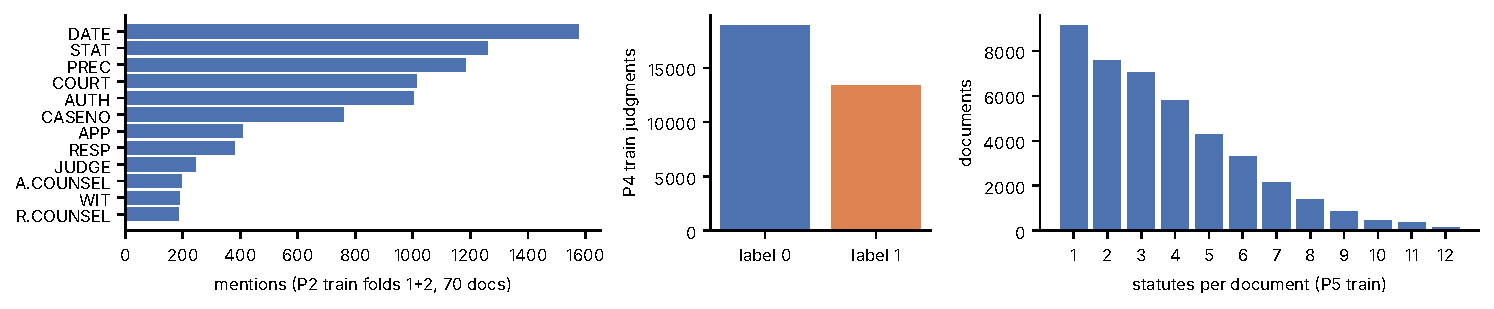
\includegraphics[width=\linewidth]{figs/data_stats.pdf}
\caption{Left: Phase-2 entity frequencies (DATE is 8.6$\times$ more frequent than R.COUNSEL). Middle: Phase-4 class balance (59/41). Right: statutes per Phase-5 training document.}
\label{fig:data}
\end{figure}

\paragraph{What the statistics implied.}
\textbf{Phase 2:} labels are imbalanced (Figure~\ref{fig:data}) and entity spans do not always align with BPE tokens: 151 gold entities (79 of them PREC) have a boundary inside a token. Converting gold spans to BIO tags and back caps strict macro-F1 at 0.987 (IO tagging: 0.971), so we used BIO. \textbf{Phase 3:} the role distribution is dominated by \texttt{RatioOfTheDecision} and \texttt{Fact}, while several roles occur only a handful of times in dev (e.g.\ 3 \texttt{Issue} sentences in CL dev), so macro-F1 is sensitive to rare roles. \textbf{Phase 4:} judgments are long, so only a few 512-token chunks fit, and the 59/41 imbalance led us to class-weighted loss and a dev-tuned decision threshold. \textbf{Phase 5:} all 100 statutes have at least 272 training positives, but the median document has 3 labels and frequency spans 272--11{,}730, so per-statute thresholds were needed. \textbf{Phase 6:} summaries are long (median 754 tokens, ratio 0.22 to the document), and only 1\% of documents fit in 768 tokens, so the source must be selected and the target truncated. \textbf{Phase 7:} queries have on average 6.4 (train) and 8.3 (dev) relevant cases, 30--33\% have more than 7, so the best attainable Micro-F1@7 is 0.643 (train) and 0.618 (dev); BM25 \cite{robertson2009bm25} over token ids gives a lexical reference of dev Micro-F1@7 0.078.

\paragraph{Preprocessing.}
One byte-level BPE tokenizer (32{,}000 entries, \texttt{</s>} = id 1) trained on the Phase-1 corpus is shared by every model. Phase~2 uses tokenizer offsets to map character spans to BIO tags (gold ends are exclusive, verified on 8{,}393 spans), sliding windows of 512 tokens with stride 384, and maps predicted tags back to character spans with whitespace trimming. Phase~3 classifies each sentence with up to 512 tokens of surrounding context. Phase~4 keeps the last 4 chunks of 512 tokens (stride 412), Phase~5 the first and last chunks (4 $\times$ 512, stride 448). Phase~6 selects 60\% of the source budget from the start and 40\% from the end (1{,}019 tokens for the encoder--decoder; 520 or 488 for models whose 1{,}024-token window also holds the summary) and appends the separator ``\texttt{\textbackslash nSummary:\textbackslash n}''. Phase~7 represents every case by up to 4 chunks of 512 tokens (two from the start, two from the end).

%=====================================================================
\section{Approach and Model Evolution}
\label{sec:approach}

\subsection{Phase 1: four foundation models}
We trained four models that each test one architectural idea while keeping the tokenizer, data mix (Supreme Court 40\%, High Courts 30\%, Acts 20\%, Tribunals 10\%), 1{,}024-token context and validation windows fixed (Table~\ref{tab:p1arch}). The \textbf{prefix-LM} attends bidirectionally inside a randomly sized prefix (30--80\% of the window) and causally after it, matching the test setting of a 512-word prompt followed by a continuation. The \textbf{encoder--decoder} encodes the prompt and decodes the continuation. The \textbf{retention model} replaces attention with multi-scale exponentially decaying retention, which allows recurrent decoding. \textbf{Bi-Scale} combines grouped-query attention, SwiGLU and RMSNorm, with sliding-window attention (256 tokens) in the lower 8 layers and global attention above. The three attention/retention models share one recipe: AdamW ($\beta$=0.9/0.95, weight decay 0.1), peak learning rate $3\times10^{-4}$ with cosine decay to $3\times10^{-5}$, 1{,}000 warmup steps, 131{,}072 tokens per step, fp16 on two T4s. Bi-Scale was trained in two stages: 71M tokens of English Wikipedia (2 h), then 283M legal tokens (8 h, peak LR $10^{-4}$), reaching validation loss 3.61 (perplexity 36.9). Continuations were sampled (Bi-Scale: temperature 0.8, top-$p$ 0.92, repetition penalty 1.15) to 128 words.

\begin{table}[H]
\centering\small
\caption{Phase-1 models (parameter counts as loaded from the final checkpoints).}
\label{tab:p1arch}
\resizebox{\linewidth}{!}{\begin{tabular}{lcccccl}
\toprule
\textbf{Model} & \textbf{Params} & \textbf{Layers} & \textbf{$d$} & \textbf{Heads} & \textbf{FFN} & \textbf{Positions / other} \\
\midrule
Prefix-LM & 109.6M & 12 & 768 & 12 & 3072 & RoPE, tied embeddings, prefix-LM mask \\
Encoder--decoder & 114.4M & 6 enc + 5 dec & 768 & 12 & 3072 & RoPE, tied embeddings \\
Retention & 109.6M & 9 & 768 & 6 & 3072 & multi-scale retention, value factor 2, RoPE \\
Bi-Scale & 144.2M & 16 & 768 & 12 q / 4 kv & 2048 (SwiGLU) & RMSNorm, RoPE, local 256 in layers 0--7, dropout 0.1 \\
\bottomrule
\end{tabular}}
\end{table}

\subsection{Transfer protocol and techniques (Phases 2--7)}
Every task model loads one of the four Phase-1 checkpoints and adds a small task head; each submission uses one adaptation technique (Figure~\ref{fig:system}). We implemented full fine-tuning; partial fine-tuning (top $k$ blocks and the final norm); BitFit \cite{benzaken2022bitfit} (biases only); LoRA \cite{hu2021lora} and rsLoRA \cite{kalajdzievski2023rslora} on attention and MLP projections; LoRMA \cite{bihany2025lorma}, which adapts weights multiplicatively ($W' = (I + BA)\,W$, ``plus'' variant); Houlsby \cite{houlsby2019parameter} and Pfeiffer \cite{pfeiffer2021adapterfusion} bottleneck adapters; prefix tuning \cite{li2021prefix} (learned key/value vectors in every attention layer); prompt tuning \cite{lester2021power} (learned input vectors); and KD \cite{hinton2015distilling}, where a student keeps an evenly spaced subset of the teacher's layers. For classification phases (2--5) the student minimises $0.5\,\mathcal{L}_{\text{task}} + 0.5\,T^2\,\mathrm{KL}$ against stored teacher logits at temperature $T=2$; in Phase~6 KD is sequence-level (teacher summaries for 800 training documents are added to the student's data); in Phase~7 the student matches the teacher's similarity distribution over candidates.

\begin{figure}[H]
\centering
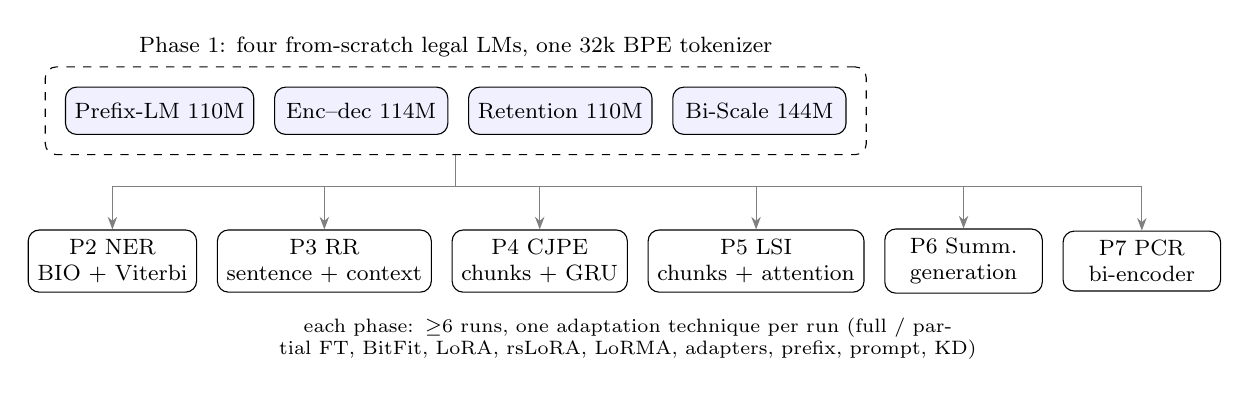
\begin{tikzpicture}[node distance=3mm and 2.5mm, every node/.style={font=\footnotesize},
  bb/.style={draw, rounded corners, fill=blue!6, minimum width=22mm, minimum height=6mm, align=center},
  ph/.style={draw, rounded corners, minimum width=20mm, minimum height=6mm, align=center},
  arr/.style={-{Stealth[length=1.6mm]}, gray}]
\node[bb] (a) {Prefix-LM 110M};
\node[bb, right=of a] (b) {Enc--dec 114M};
\node[bb, right=of b] (c) {Retention 110M};
\node[bb, right=of c] (d) {Bi-Scale 144M};
\node[draw, dashed, rounded corners, fit=(a)(b)(c)(d), inner sep=2.5mm, label={[font=\footnotesize]above:Phase 1: four from-scratch legal LMs, one 32k BPE tokenizer}] (p1) {};
\node[ph, below=12mm of a, xshift=-6mm] (p2) {P2 NER\\BIO + Viterbi};
\node[ph, right=of p2] (p3) {P3 RR\\sentence + context};
\node[ph, right=of p3] (p4) {P4 CJPE\\chunks + GRU};
\node[ph, right=of p4] (p5) {P5 LSI\\chunks + attention};
\node[ph, right=of p5] (p6) {P6 Summ.\\generation};
\node[ph, right=of p6] (p7) {P7 PCR\\bi-encoder};
\foreach \n in {p2,p3,p4,p5,p6,p7} \draw[arr] (p1.south) -- ++(0,-4mm) -| (\n.north);
\node[below=2mm of p4.south east, font=\scriptsize, text width=13cm, align=center] {each phase: $\geq$6 runs, one adaptation technique per run (full / partial FT, BitFit, LoRA, rsLoRA, LoRMA, adapters, prefix, prompt, KD)};
\end{tikzpicture}
\caption{Overall system: the Phase-1 backbones are adapted separately for each task.}
\label{fig:system}
\end{figure}

\subsection{Task models}
\textbf{Phase 2 (NER)} tags tokens with BIO labels from a linear head; predictions from overlapping windows are merged, and we compared greedy (``lenient'') decoding with Viterbi decoding that forbids invalid transitions (runs ending in \texttt{\_viterbi} re-decode the same trained weights). The KD student is an 8-layer Bi-Scale distilled from the full fine-tuned Bi-Scale. \textbf{Phase 3 (RR)} classifies each sentence from its pooled representation inside a 512-token context window. \textbf{Phase 4 (CJPE)} encodes up to 4 chunks, pools each (mean for bidirectional models, mean + last token for causal ones), combines the chunk vectors with a GRU and predicts the label with a threshold tuned on dev. \textbf{Phase 5 (LSI)} uses attention pooling over chunks, a 100-way sigmoid head initialised to the label prior, balanced positive weights (capped at 10) and per-statute thresholds tuned on dev, with at least one statute per document. \textbf{Phase 6} generates with each backbone directly: the encoder--decoder decodes from the encoded source, the other three continue the source prefix; decoding is greedy with repetition penalty 1.2, no repeated 4-grams and 300--800 (encoder--decoder) or 250--480 new tokens. \textbf{Phase 7} is a bi-encoder: chunk vectors (mean pooling; mean + last token for causal models) are max-pooled into a case vector, candidates are ranked by cosine similarity, and training uses InfoNCE \cite{oord2018cpc,karpukhin2020dpr} with temperature 0.05 over one relevant case, 7 negatives (4 from the BM25 top-50, 3 random) and in-batch negatives, masking in-batch cases that are relevant to the query.

\paragraph{What failed or changed.} Phase-3 runs on the encoder--decoder with prefix tuning reached only 0.20 dev macro-F1, and in Phase~7 both encoder-only encoder--decoder runs (LoRMA, prefix) scored below the BM25 reference on the test set, while full and partial fine-tuning of the same pipeline worked. In Phase~5, prompt tuning on the encoder--decoder (0.11 dev macro-F1) and an untuned global threshold (which predicted 99.7 statutes per document in our smoke tests) were replaced by per-statute thresholds. In Phase~4, argmax decisions under-predicted label 1 (the full fine-tuned prefix-LM scored 0.41 with argmax and 0.61 with a tuned threshold).

%=====================================================================
\section{Experiments and Implementation Details}
\label{sec:experiments}
All task runs used a Kaggle notebook with two T4 GPUs: one background process per GPU, fp16 autocast, AdamW with gradient clipping at 1.0, linear warmup and decay, and a per-run wall-clock cap; a notebook-level guard shortened later runs so that every run finished inside the 12-hour session. After every epoch the run is scored on held-out labelled data and the best epoch's trainable weights are kept. Table~\ref{tab:hparams} lists the settings shared by all runs of a phase (method-specific multipliers scale the learning rate of new parameters).

\begin{table}[H]
\centering\small
\caption{Training settings shared by all runs of each phase.}
\label{tab:hparams}
\resizebox{\linewidth}{!}{\begin{tabular}{lcccccc}
\toprule
 & \textbf{P2 NER} & \textbf{P3 RR} & \textbf{P4 CJPE} & \textbf{P5 LSI} & \textbf{P6 Summ.} & \textbf{P7 PCR} \\
\midrule
Peak LR & $5\times10^{-5}$ & $5\times10^{-4}$ & $5\times10^{-4}$ & $5\times10^{-4}$ & $5\times10^{-4}$ & $2\times10^{-4}$ \\
Batch $\times$ accum. & 8 $\times$ 1 & 8 $\times$ 1 & 4 $\times$ 4 & 4 $\times$ 4 & 4 $\times$ 4 & 4 $\times$ 2 queries \\
Epochs (cases/epoch) & 10 & 15 & 5 (4{,}000) & 6 (8{,}000) & 10 (3{,}000) & 6 (all 817) \\
Warmup / weight decay & 10\% / 0.01 & 10\% / 0.01 & 6\% / 0.01 & 6\% / 0.01 & 5\% / 0.01 & 10\% / 0.01 \\
Time cap per run & 60 min & 30 min & 50 min & 85 min & 100 min & 100 min \\
Input & 512 / stride 384 & 512 context & 4 $\times$ 512, last & 4 $\times$ 512, head+tail & 1{,}019 or 520 src & 4 $\times$ 512, head+tail \\
Loss / extras & CE, BIO & CE & weighted CE & weighted BCE & CE, smoothing 0.1 & InfoNCE $\tau$=0.05 \\
Model selection & val macro-F1 & dev macro-F1 & dev macro-F1 & dev tuned macro-F1 & val loss & dev Micro-F1@7 \\
\bottomrule
\end{tabular}}
\end{table}

\paragraph{Local evaluation.} Phases 3, 4, 5 and 7 use the official labelled dev splits with the competition metric. Phase~2 holds out 15\% of the training documents (seed 0) and computes strict macro-F1 on character spans. Phase~6 has no dev split, so 200 training documents (seed 0) are held out; validation loss selects the epoch and ROUGE on 30 of them is reported (BERTScore was not computed locally).

%=====================================================================
\section{Results}
\label{sec:results}
Tables~\ref{tab:p2}--\ref{tab:p7} report every run with its local score (from the run logs) and its Codabench score; Figure~\ref{fig:curves} shows the learning curves.

\begin{table}[H]
\centering\small
\caption{Phase 2 (L-NER) runs: local validation macro-F1/P/R (strict spans), decoding of the BIO tags, training minutes and Codabench score. Rows ending in \texttt{\_viterbi} re-decode a trained run's weights with Viterbi.}
\label{tab:p2}
\resizebox{\linewidth}{!}{\begin{tabular}{lllcccccc}
\toprule
\textbf{Run} & \textbf{Technique / backbone} & \textbf{Trainable / total} & \textbf{Decode} & \textbf{Val F1} & \textbf{Val P} & \textbf{Val R} & \textbf{Min} & \textbf{Codabench} \\
\midrule
\texttt{prefixlm\_lorma\_viterbi} & LoRMA ($r$=16) / Prefix-LM & 2.67M / 112.3M & viterbi & 0.5328 & 0.5513 & 0.5303 & 0.0 & \textbf{0.5126} \\
\texttt{kd\_student} & KD student (8 layers) / Bi-Scale & 89.70M / 89.7M & viterbi & 0.5123 & 0.5309 & 0.5071 & 5.2 & 0.4607 \\
\texttt{prefixlm\_bitfit} & BitFit / Prefix-LM & 0.12M / 109.7M & viterbi & 0.5079 & 0.5232 & 0.5093 & 7.3 & 0.4440 \\
\texttt{biscale\_full\_viterbi} & full FT / Bi-Scale & 149.49M / 149.5M & viterbi & 0.4942 & 0.5093 & 0.4887 & 0.0 & 0.4933 (failed) \\
\texttt{arch4\_adapter\_viterbi} & Houlsby adapter (64) / Retention & 7.11M / 116.7M & viterbi & 0.4648 & 0.4902 & 0.4574 & 0.0 & 0.4619 \\
\texttt{prefixlm\_lorma} & LoRMA ($r$=16) / Prefix-LM & 2.67M / 112.3M & lenient & 0.4377 & 0.4064 & 0.4862 & 9.3 & 0.4036 \\
\texttt{biscale\_full} & full FT / Bi-Scale & 149.49M / 149.5M & lenient & 0.4323 & 0.4142 & 0.4648 & 10.5 & -- \\
\texttt{arch4\_adapter} & Houlsby adapter (64) / Retention & 7.11M / 116.7M & lenient & 0.3642 & 0.3422 & 0.4002 & 7.2 & -- \\
\texttt{encdec\_lora\_viterbi} & LoRA ($r$=16) / Enc--dec & 1.20M / 68.3M & viterbi & 0.1828 & 0.2221 & 0.1902 & 0.0 & -- \\
\texttt{encdec\_lora} & LoRA ($r$=16) / Enc--dec & 1.20M / 68.3M & lenient & 0.1236 & 0.1217 & 0.1578 & 3.9 & 0.1181 \\
\bottomrule
\end{tabular}}
\end{table}

\begin{table}[H]
\centering\small
\caption{Phase 3 (rhetorical roles) runs: local dev macro-F1 (both domains pooled, CL, IT) and Codabench score.}
\label{tab:p3}
\resizebox{\linewidth}{!}{\begin{tabular}{lllccccc}
\toprule
\textbf{Run} & \textbf{Technique / backbone} & \textbf{Trainable / total} & \textbf{Dev comb.} & \textbf{Dev CL} & \textbf{Dev IT} & \textbf{Min} & \textbf{Codabench} \\
\midrule
\texttt{r3\_rslora\_arch4} & rsLoRA ($r$=32) / Retention & 5.12M / 114.7M & 0.4268 & 0.3459 & 0.4606 & 29.0 & 0.4489 \\
\texttt{r1\_lorma\_prefixlm} & LoRMA ($r$=16) / Prefix-LM & 3.15M / 112.8M & 0.4196 & 0.3704 & 0.4202 & 25.4 & \textbf{0.4941} \\
\texttt{r6\_kd\_student} & KD student (8 layers) / Prefix-LM & 81.78M / 81.8M & 0.3860 & 0.3237 & 0.3991 & 19.5 & 0.4536 \\
\texttt{r4\_prompt\_biscale} & prompt tuning (32) / Bi-Scale & 0.72M / 144.9M & 0.3579 & 0.3128 & 0.3660 & 30.1 & 0.4067 \\
\texttt{r2\_lora\_encdec} & LoRA ($r$=16) / Enc--dec & 1.68M / 68.8M & 0.2768 & 0.2628 & 0.2541 & 12.5 & 0.3142 \\
\texttt{r5\_prefix\_encdec} & prefix tuning (16) / Enc--dec & 0.64M / 67.7M & 0.1965 & 0.1653 & 0.2064 & 9.2 & 0.2107 \\
\bottomrule
\end{tabular}}
\end{table}

\begin{table}[H]
\centering\small
\caption{Phase 4 (CJPE) runs: local dev macro-F1 with the threshold tuned on dev and with argmax, the threshold, and Codabench score. The last four runs have no local log in our backup, so only their Codabench scores are shown.}
\label{tab:p4}
\resizebox{\linewidth}{!}{\begin{tabular}{lllccccc}
\toprule
\textbf{Run} & \textbf{Technique / backbone} & \textbf{Trainable / total} & \textbf{Dev (thr.)} & \textbf{Dev (argmax)} & \textbf{Thr.} & \textbf{Min} & \textbf{Codabench} \\
\midrule
\texttt{r3\_partial\_arch4} & partial FT (top 3) / Retention & 29.03M / 110.3M & 0.6467 & 0.5999 & 0.432 & 23.5 & 0.6123 \\
\texttt{r6\_kd\_student} & KD student (8 layers) / Prefix-LM & 81.78M / 81.8M & 0.6397 & 0.5858 & 0.279 & 28.6 & \textbf{0.6224} \\
\texttt{r7\_full\_prefixlm} & full FT / Prefix-LM & 110.13M / 110.1M & 0.6113 & 0.4071 & 0.325 & 51.4 & 0.5658 \\
\texttt{r5\_bitfit\_prefixlm} & BitFit / Prefix-LM & 0.60M / 110.1M & 0.5842 & 0.5794 & 0.504 & 51.2 & 0.5477 \\
\texttt{r4\_adapter\_biscale} & Houlsby adapter (64) / Bi-Scale & 3.86M / 148.0M & 0.3867 & 0.3333 & 0.477 & 48.3 & 0.3915 \\
\texttt{r2b\_full\_encdec\_lc} & full FT / Enc--dec (\texttt{\_lc} variant) & -- & -- & -- & -- & -- & 0.5563 \\
\texttt{r2\_full\_encdec} & full FT / Enc--dec & -- & -- & -- & -- & -- & 0.5568 \\
\texttt{r1b\_lorma\_prefixlm\_lc} & LoRMA ($r$=16) / Prefix-LM (\texttt{\_lc} variant) & -- & -- & -- & -- & -- & 0.4740 \\
\texttt{r1\_lorma\_prefixlm} & LoRMA ($r$=16) / Prefix-LM & -- & -- & -- & -- & -- & 0.4146 \\
\bottomrule
\end{tabular}}
\end{table}

\begin{table}[H]
\centering\small
\caption{Phase 5 (LSI) runs: local dev macro/micro-F1 with per-statute thresholds, statutes predicted per test document, and Codabench score.}
\label{tab:p5}
\resizebox{\linewidth}{!}{\begin{tabular}{lllccccc}
\toprule
\textbf{Run} & \textbf{Technique / backbone} & \textbf{Trainable / total} & \textbf{Dev macro} & \textbf{Dev micro} & \textbf{Stat./doc} & \textbf{Min} & \textbf{Codabench} \\
\midrule
\texttt{r8\_full\_prefixlm} & full FT / Prefix-LM & 110.08M / 110.1M & 0.3788 & 0.4711 & 5.01 & 83.7 & \textbf{0.3582} \\
\texttt{r6\_kd\_student} & KD student (8 layers) / Prefix-LM & 81.73M / 81.7M & 0.3643 & 0.4577 & 5.22 & 61.0 & 0.3531 \\
\texttt{r1\_lorma\_prefixlm} & LoRMA ($r$=16) / Prefix-LM & 3.10M / 112.7M & 0.3569 & 0.4481 & 5.49 & 87.6 & 0.3433 \\
\texttt{r3\_partial\_arch4} & partial FT (top 3) / Retention & 29.18M / 110.4M & 0.3533 & 0.4493 & 5.42 & 56.6 & 0.3334 \\
\texttt{r7\_prefix\_prefixlm} & prefix tuning (16) / Prefix-LM & 0.74M / 110.4M & 0.3159 & 0.4064 & 6.29 & 60.1 & 0.3017 \\
\texttt{r4\_adapter\_biscale} & Houlsby adapter (64) / Bi-Scale & 4.01M / 148.2M & 0.3092 & 0.4013 & 6.59 & 90.7 & 0.2948 \\
\texttt{r2\_full\_encdec} & full FT / Enc--dec & 67.55M / 67.6M & 0.1828 & 0.2326 & 12.38 & 41.8 & 0.1698 \\
\texttt{r5\_prompt\_encdec} & prompt tuning (32) / Enc--dec & 0.47M / 67.6M & 0.1105 & 0.1401 & 23.37 & 37.9 & 0.1007 \\
\bottomrule
\end{tabular}}
\end{table}

\begin{table}[H]
\centering\small
\caption{Phase 6 (summarization) runs: ROUGE on 30 held-out training documents, mean summary length in words (references: 874), and Codabench BERTScore F1.}
\label{tab:p6}
\resizebox{\linewidth}{!}{\begin{tabular}{lllcccccc}
\toprule
\textbf{Run} & \textbf{Technique / backbone} & \textbf{Trainable / total} & \textbf{R-1} & \textbf{R-2} & \textbf{R-L} & \textbf{Words} & \textbf{Min} & \textbf{Codabench} \\
\midrule
\texttt{r2\_lora\_prefixlm} & LoRA ($r$=16) / Prefix-LM & 2.36M / 112.0M & 0.3874 & 0.1587 & 0.2065 & 331 & 39.3 & \textbf{0.8333} \\
\texttt{r5\_prefix\_prefixlm} & prefix tuning (16) / Prefix-LM & 0.29M / 109.9M & 0.3645 & 0.1377 & 0.1901 & 334 & 30.8 & 0.8299 \\
\texttt{r3\_houlsby\_arch4} & Houlsby adapter (64) / Retention & 1.78M / 111.4M & 0.3427 & 0.1199 & 0.1794 & 280 & 34.4 & 0.8293 \\
\texttt{r7\_prompt\_biscale} & prompt tuning (32) / Bi-Scale & 0.02M / 144.2M & 0.3334 & 0.0957 & 0.1724 & 410 & 60.6 & 0.8074 \\
\texttt{r6\_kd\_encdec\_student} & KD student (4+3 layers) / Enc--dec & 81.29M / 81.3M & 0.2972 & 0.0744 & 0.1589 & 288 & 30.0 & 0.8153 \\
\texttt{r1\_lorma\_encdec} & LoRMA ($r$=16) / Enc--dec & 2.92M / 117.3M & 0.2958 & 0.0755 & 0.1606 & 294 & 44.0 & 0.8155 \\
\texttt{r4\_pfeiffer\_encdec} & Pfeiffer adapter (128) / Enc--dec & 2.17M / 116.5M & 0.2908 & 0.0749 & 0.1567 & 295 & 34.0 & 0.8119 \\
\bottomrule
\end{tabular}}
\end{table}


\begin{table}[H]
\centering\small
\caption{Phase 7 (PCR) runs: Codabench Micro-F1@7 on the 237 test queries.}
\label{tab:p7}
\resizebox{\linewidth}{!}{\begin{tabular}{lllcc}
\toprule
\textbf{Run} & \textbf{Technique / backbone} & \textbf{Trainable / total} & \textbf{Dev F1@7} & \textbf{Codabench F1@7} \\
\midrule
\texttt{p1\_full} & full FT (KD teacher) / Prefix-LM & 109.63M / 109.6M & -- & \textbf{0.2593} \\
\texttt{p6\_kd\_student} & KD student (8 layers) / Prefix-LM & 81.28M / 81.3M & -- & 0.2463 \\
\texttt{p2\_partial} & partial FT (top 3) / Retention & 28.34M / 109.6M & 0.2657 & 0.2221 \\
\texttt{p5\_prompt} & prompt tuning (16) / Bi-Scale & 0.01M / 144.2M & -- & 0.1122 \\
\texttt{p3\_lorma} & LoRMA ($r$=16) / Enc--dec encoder & 1.33M / 68.4M & -- & 0.0307 \\
\texttt{p4\_prefix} & prefix tuning (16) / Enc--dec encoder & 0.15M / 67.3M & -- & 0.0089 \\
\midrule
BM25 reference & lexical, token ids & -- & 0.0778 & -- \\
\bottomrule
\end{tabular}}
\end{table}

\begin{figure}[H]
\centering
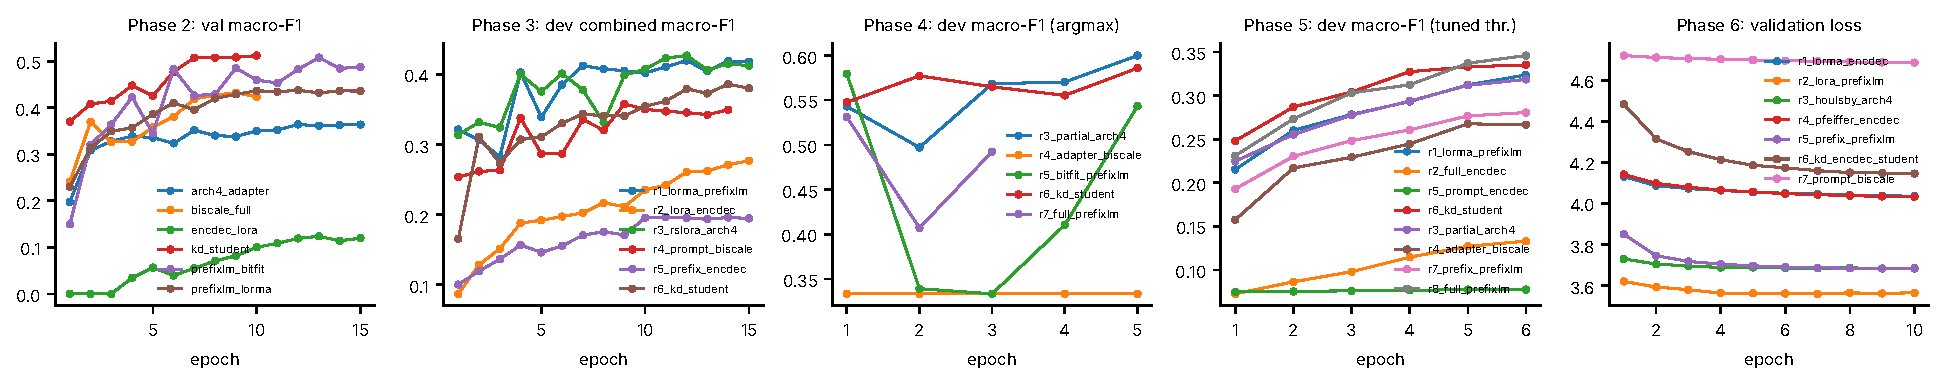
\includegraphics[width=\linewidth]{figs/learning_curves.pdf}
\caption{Local metric per epoch for every run of Phases 2--6 (Phase 6: validation loss, lower is better).}
\label{fig:curves}
\end{figure}

\paragraph{Which systems won and why.}
\textbf{Phase 1:} the retention model gave the best continuation BERTScore (0.835), ahead of Bi-Scale (0.827) and the encoder--decoder (0.807); our other submissions (decoder-only and prefix-LM variants) scored 0.821--0.831. All lie within 0.03, because BERTScore of fluent legal prose against a reference continuation saturates quickly. \textbf{Phases 2--7:} the \textbf{prefix-LM} produced the winning test submission in all six phases (NER, rhetorical roles, judgment prediction through its KD student, statutes, summarization and retrieval). We attribute this to its pretraining objective: it already learned bidirectional attention over a prefix, so its hidden states summarise a whole span or chunk, whereas the causal retention and Bi-Scale models must route that information to the last position. Decision rules mattered as much as the backbone: Viterbi decoding raised the same prefix-LM LoRMA NER model from 0.404 to 0.513 on the test set by removing invalid BIO transitions, and in Phase~4 a dev-tuned threshold turned an argmax score of 0.41 into 0.61 on dev. \textbf{KD students} were close to or better than their teachers on the test sets: Phase 4 0.622 vs.\ 0.612, Phase 5 0.353 vs.\ 0.343, Phase 6 0.815 vs.\ 0.816, Phase 7 0.246 vs.\ 0.259, with 26--31\% fewer parameters than the teacher, which suggests that the teacher's soft targets regularise training on these small datasets. Dev and test rankings mostly agreed; the exceptions were Phase 3, where rsLoRA on the retention model led on dev (0.427) but LoRMA on the prefix-LM led on test (0.494 vs.\ 0.449), and Phase 2, where the KD student led on our 15\% validation split (0.512) but not on test (0.461), consistent with the small NER validation set (about 10 documents). The weakest runs were consistently those that keep the \textbf{encoder--decoder's encoder} frozen and train few parameters (test: NER LoRA 0.118, RR prefix 0.211, LSI prompt 0.101, PCR LoRMA 0.031 and prefix 0.009). This encoder was only trained to feed a decoder through cross-attention, so its states are not directly usable as features without updating it; even full fine-tuning of it stayed behind the other backbones (LSI 0.170, CJPE 0.557).

%=====================================================================
\section{Error Analysis and Discussion}
\label{sec:error}
\textbf{Phase 2.} Strict matching punishes boundary errors: PREC and STAT spans are long and their boundaries often fall inside a BPE token (79 PREC entities), and Viterbi decoding helped mainly by removing invalid BIO transitions (orphan I-tags): the same prefix-LM LoRMA weights scored 0.404 with greedy decoding and 0.513 with Viterbi on the test set. \textbf{Phase 3.} Predictions collapse onto the two majority roles: on the 2{,}197 test sentences one run predicted \texttt{RatioOfTheDecision} for 1{,}816 and \texttt{Fact} for 371, leaving nine roles almost unpredicted; IT dev scores were higher than CL in five of the six runs. \textbf{Phase 4.} Keeping only the last 4 chunks drops the facts at the start of long judgments, and argmax decisions under-predict label 1, so the dev-tuned threshold (0.28--0.50) moved macro-F1 by up to 0.20. \textbf{Phase 5.} The weakest statutes on dev (F1 $\leq$ 0.13 in the final runs: ids 0, 2, 8, 27, 41) have 83--205 dev positives and at least 272 training positives, so the failures are not caused by unseen labels; with per-statute thresholds the stronger runs predict 5--7 statutes per test document (the training average is 3.6), while the weak encoder--decoder runs predict 12--23. \textbf{Phase 6.} All models produce summaries one third to one half as long as the references (280--410 words vs.\ 874), so recall-oriented metrics are capped; examples show fluent, case-specific openings with factual slips (wrong party roles). \textbf{Phase 7.} About a third of the queries have more than 7 relevant cases, so recall@7 is capped; the fine-tuned dense retrievers reach about three times the BM25 dev reference, but only methods that update the backbone get there.

\paragraph{What the metrics miss.} BERTScore \cite{zhang2020bertscore} and ROUGE \cite{lin2004rouge} reward lexical overlap and fluency but not legal correctness (party roles, outcomes, cited sections); macro-F1 in Phase~3 is dominated by roles with a handful of dev sentences; Micro-F1@7 ignores ranking order within the top 7.

\paragraph{Limitations and next steps.} Each run was trained once (no seeds), so differences below about 0.01--0.02 are within noise; Phase-6 BERTScore was not measured locally; context is limited to 1{,}024 tokens. Next steps: hierarchical encoders over all chunks for Phases 4--7, cross-encoder re-ranking of the Phase-7 top-50, and length control in Phase~6.

%=====================================================================
\section{Conclusion}
\label{sec:conclusion}
Three choices moved the metrics most: a bidirectional pretraining objective (the prefix-LM transferred best), task-specific decision rules (Viterbi decoding, tuned thresholds, top-$k$ retrieval with masked in-batch negatives), and updating the backbone rather than only adding a few parameters when the backbone was not pretrained for the target use. Distillation into smaller students was a cheap and reliable way to keep most of the performance. The main lesson is that with a small from-scratch model and a fixed compute budget, how a model's pretraining objective matches the downstream use matters more than which parameter-efficient method is applied.

%=====================================================================
\clearpage
\bibliographystyle{plain}
\bibliography{references}

%=====================================================================
\clearpage
\section*{LLM Usage Declaration}
\medskip\noindent\textbf{Q1. Which LLM(s) did you use?} Claude (Anthropic).

\medskip\noindent\textbf{Q2. For each row, mark Yes or No and state the purpose in one short phrase.} ``Yes'' is acceptable only for the uses permitted by the capstone document.
\begin{table}[H]
\centering\small
\begin{tabular}{>{\raggedright\arraybackslash}p{4.6cm}c>{\raggedright\arraybackslash}p{8.2cm}}
\toprule
\textbf{Part} & \textbf{Used LLM?} & \textbf{Purpose of using the LLM} \\
\midrule
Understanding concepts / papers & Yes & Explaining PEFT methods (LoRA, LoRMA, adapters, prefix/prompt tuning) and the architectures in the papers \\
Ideation / brainstorming at a high level & No & -- \\
Debugging small ancillary snippets & Yes & Locating the cause of errors in small helper snippets \\
Plotting / visualization code & No & -- \\
Grammar / writing style of the report & Yes & Correcting grammar and improving clarity of sentences \\
Report structure / section wording & Yes & Organising the report sections and wording of headings \\
Designing the model architecture & No & -- \\
Hyperparameter search / tuning & No & -- \\
Analysis of results / conclusions & No & -- \\
Writing the core training / inference code & No & -- \\
Other (specify) & No & -- \\
\bottomrule
\end{tabular}
\end{table}

\medskip\noindent\textbf{Q3. Did you refer to sources other than lecture slides and an LLM?} Yes. English Wikipedia text \cite{wikipedia} (71M tokens) was used for the first stage of Bi-Scale pretraining only; the instructor permitted this in an announcement on the course Discord. No other external data was used.

\medskip\noindent\textbf{Q4. Apart from any permitted LLM use, what was your contribution?} I decided what to train in every phase: which of the four Phase-1 backbones to pair with which adaptation method, so that each phase compared genuinely different approaches. I chose every hyperparameter myself, including learning rates and their multipliers, batch sizes and gradient accumulation, the number of epochs and cases per epoch, LoRA/LoRMA ranks, adapter sizes, and the numbers of prefix and prompt tokens. I also chose the input settings, such as chunk lengths, the number of chunks and which part of a long judgment to keep, and the generation and retrieval settings. I decided how long each model should train, set the per-run time budgets and arranged the runs on the two GPUs so that everything finished within a Kaggle session. For knowledge distillation I chose the teacher and how many layers the student keeps. I ran all experiments on Kaggle, monitored the logs, and fixed settings when a run did not fit, for example the context length in Phase 6. I checked the local and Codabench results of every run and decided which submissions to keep. Two things I tried failed: prefix tuning and prompt tuning on the frozen encoder--decoder encoder (0.20 dev macro-F1 in Phase~3, 0.11 in Phase~5), from which I concluded that an encoder trained only to feed a decoder must be updated to be useful as a feature extractor; and argmax decisions in Phase~4 and a single global threshold in Phase~5, which led me to tune thresholds on dev for every classification phase. I take responsibility for all results reported here and can explain how each was produced.

\end{document}
